\documentclass[border=6pt]{standalone}
\usepackage{amsmath,amssymb}
\usepackage{tikz}
\usetikzlibrary{arrows.meta,calc,decorations.pathreplacing,patterns,shapes.geometric,positioning,shadings,plotmarks}

\begin{document}
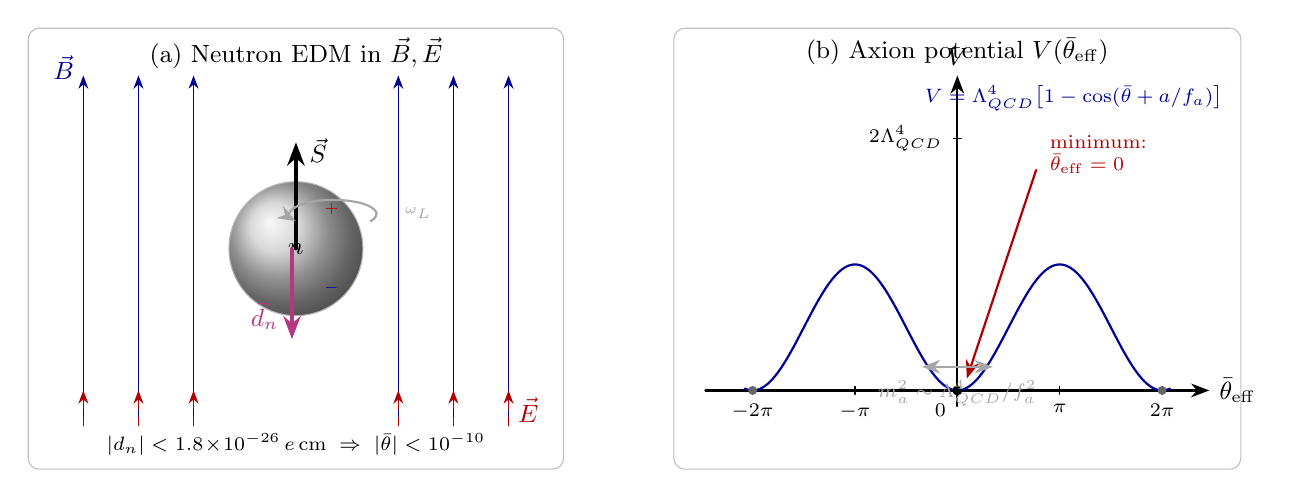
\begin{tikzpicture}[>=Stealth, line cap=round, line join=round]

% =====================================================================
% LEFT PANEL: neutron with EDM in B field (Ramsey-style schematic)
% =====================================================================
\begin{scope}[shift={(0,0)}]

  % Panel frame
  \draw[rounded corners=4pt, gray!50, thin] (-3.4,-2.6) rectangle (3.4,3.0);
  \node[anchor=north] at (0,3.0) {\small (a) Neutron EDM in $\vec B,\vec E$};

  % Background B-field arrows (uniform field pointing up)
  \foreach \x in {-2.7,-2.0,-1.3,1.3,2.0,2.7}{
    \draw[->, blue!55!black, thin] (\x,-2.0) -- (\x,2.4);
  }
  \node[blue!55!black] at (-2.95,2.5) {\small $\vec B$};

  % Electric field (smaller arrows on side)
  \foreach \x in {-2.7,-2.0,-1.3,1.3,2.0,2.7}{
    \draw[->, red!70!black, thin, dashed] (\x,-2.05) -- (\x,-1.6);
  }
  \node[red!70!black] at (2.95,-1.85) {\small $\vec E$};

  % Neutron (sphere)
  \shade[ball color=gray!40] (0,0.2) circle (0.85);
  \draw[gray!60] (0,0.2) circle (0.85);
  \node at (0,0.2) {\small $n$};

  % Spin arrow (along B)
  \draw[->, very thick, black] (0,0.2) -- (0,1.55);
  \node[anchor=west] at (0.05,1.45) {\small $\vec S$};

  % EDM vector (slightly tilted to suggest dipole, parallel to spin)
  \draw[->, very thick, magenta!70!black] (-0.05,0.2) -- (-0.05,-0.95);
  \node[anchor=east, magenta!70!black] at (-0.1,-0.65) {\small $\vec d_n$};

  % Charge separation hint (+ and -)
  \node[red!70!black] at (0.45,0.7) {\tiny $+$};
  \node[blue!70!black] at (0.45,-0.3) {\tiny $-$};

  % Larmor precession arc
  \draw[->, gray!70, thick] (0.95,0.55) arc[start angle=-30, end angle=210, x radius=0.55, y radius=0.18];
  \node[gray!70] at (1.55,0.65) {\tiny $\omega_L$};

  % Bound on d_n
  \node[anchor=south] at (0,-2.55)
    {\scriptsize $|d_n|<1.8\!\times\!10^{-26}\,e\,\mathrm{cm}\;\Rightarrow\;|\bar\theta|<10^{-10}$};
\end{scope}

% =====================================================================
% RIGHT PANEL: axion potential V(theta-bar) cosine, min at 0
% =====================================================================
\begin{scope}[shift={(8.4,0)}]

  % Panel frame
  \draw[rounded corners=4pt, gray!50, thin] (-3.6,-2.6) rectangle (3.6,3.0);
  \node[anchor=north] at (0,3.0) {\small (b) Axion potential $V(\bar\theta_{\mathrm{eff}})$};

  % Axes
  \draw[->, thick] (-3.2,-1.6) -- (3.2,-1.6) node[anchor=west] {\small $\bar\theta_{\mathrm{eff}}$};
  \draw[->, thick] (0,-1.8) -- (0,2.4) node[anchor=south] {\small $V$};

  % x-axis tick labels: -2pi, -pi, 0, pi, 2pi
  \foreach \x/\lab in {-2.6/{-2\pi},-1.3/{-\pi},1.3/{\pi},2.6/{2\pi}}{
    \draw (\x,-1.55) -- (\x,-1.65);
    \node[anchor=north, font=\scriptsize] at (\x,-1.65) {$\lab$};
  }
  \node[anchor=north east, font=\scriptsize] at (-0.02,-1.65) {$0$};

  % y-axis tick: 2 Lambda^4
  \draw (-0.05,1.6) -- (0.05,1.6);
  \node[anchor=east, font=\scriptsize] at (-0.07,1.6) {$2\Lambda_{QCD}^4$};

  % V = Lambda^4 (1 - cos x)  with x in [-2pi, 2pi], scale: 1.3 per pi, height 0.8 per Lambda^4
  % so V_plot(x) = 0.8 * (1 - cos(pi*x/1.3)) - 1.6  (baseline at -1.6)
  % Plot using domain in TikZ
  \draw[thick, blue!60!black, smooth, samples=200, domain=-2.7:2.7]
    plot (\x, {0.8*(1 - cos( deg(pi*\x/1.3) )) - 1.6});

  % Mark minima at theta_eff = 0, +-2pi
  \filldraw[black] (0,-1.6) circle (1.6pt);
  \filldraw[black!60] (-2.6,-1.6) circle (1.4pt);
  \filldraw[black!60] (2.6,-1.6) circle (1.4pt);

  % Highlight global minimum
  \draw[->, thick, red!70!black] (1.0,1.2) -- (0.12,-1.45);
  \node[anchor=west, red!70!black, font=\scriptsize, align=left] at (1.05,1.4)
    {minimum:\\$\bar\theta_{\mathrm{eff}}=0$};

  % Curvature near minimum -> axion mass
  \draw[<->, thick, gray!70] (-0.45,-1.30) -- (0.45,-1.30);
  \node[anchor=north, gray!70, font=\scriptsize] at (0,-1.35) {$m_a^2 \sim \Lambda_{QCD}^4/f_a^2$};

  % Formula label
  \node[anchor=north east, font=\scriptsize, blue!60!black, align=right]
    at (3.5,2.4) {$V=\Lambda_{QCD}^4\bigl[1-\cos(\bar\theta+a/f_a)\bigr]$};

\end{scope}

\end{tikzpicture}
\end{document}
